\newpage
\section*{Часть 2}
	\paragraph{1)}
	Цель работы:  \\

	1) Изучение команд для просмотра типа файлов и содержимого файлов. \\

	2) Изучение команд для управления правами доступа к файлам и каталогам. \\

	3) Изучение команд для ввода/вывода данных. Перенаправление ввода/вывода. \\
	\subsection*{5 Просмотр содержимого файлов}
	
		\paragraph{1)}
		Просмотреть тип файлов из папки «Произведение автора» и файла, который извлекли из архива .zip (п.3 задания 2). 
		\\
	 	Для просмотра типа файла можно использовать несколько вариантов команд, 		одни из 			которых \textit{file <name>} и \textit{file} с ключом 			\textit{--mime-type} . Для 			поиска файлов в папке Произведения 				Лермонтова воспользуемся формой \textit{./				Произведения\ 				Лермонтова/*} , где * обозначает любой файл.
	\\
	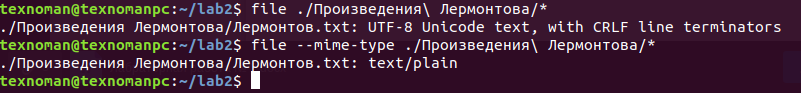
\includegraphics[width=\textwidth]{110.png} %из Произведения Лермонтова%
	\\
	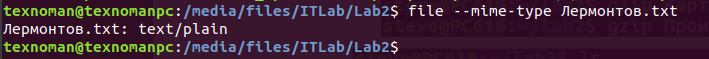
\includegraphics[width=\textwidth]{111.png} %из Lab2%
	\\
	
		\paragraph{2)}
		Просмотреть величину файлов. Выбрать наименьший пригодный для вывода на экран файл. Воспользоваться редактором cat. Вывести на экран содержимое файла, сжав пустые строки и пронумеровав строки с текстом (Использовать одну команду). 
		\\
		Для просмотра величины файла была выбрана команда \textit{ls -s <name>}, 		где ключ \textit{-s} означает size. \\
	Выбирать особо не из чего, поэтому был выбран файл \textit{Лермонтов.txt}.\\
	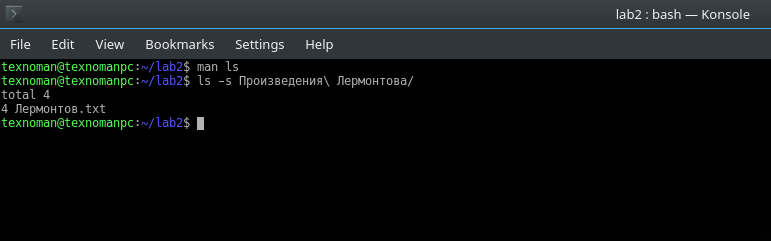
\includegraphics[width=\textwidth]{picture20.png} 
	\\
		Далее, чтобы вывести текст на экран без пустых строк использовалась команда 	\textit{cat -b <(grep ' ' <name>)}, где \textit{-b} отображает номер строк, 		стрелка потока обозначает последовательность действий, а операция в  				\textit{grep} не дает возможность отображению пустых страк, так как в них 			отсутствуют знаки пробела.\\
	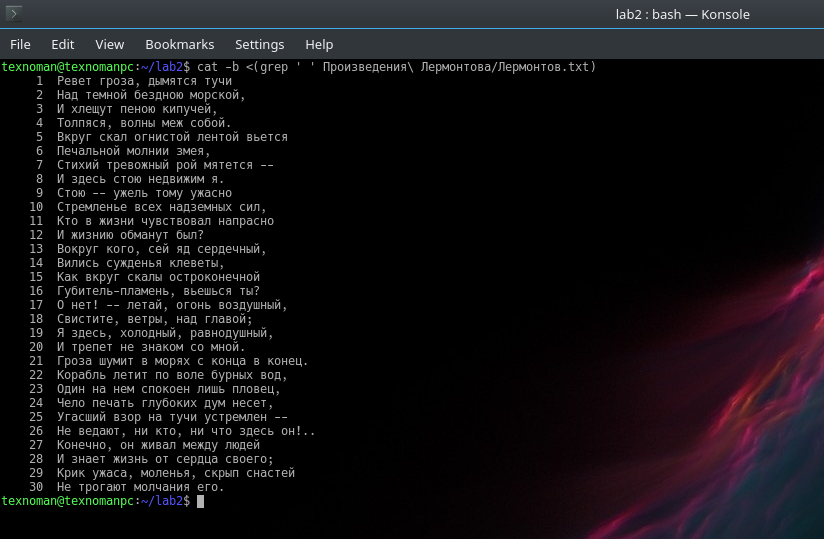
\includegraphics[width=\textwidth]{picture21.png} 
	\\
	
		\paragraph{3)}
		Вывести любое произведение автора с помощью редактора more. Отобразить полуэкран (11 строк) текста из файла и вывести номер текущей строки (одной командой). 
		\\
		За неимением других вариантов было выбрано произведение "Гроза". Для вывода 	первых 11 строк с помощью команды \textit{more} следует добавить \textit{-11}.
	\\
	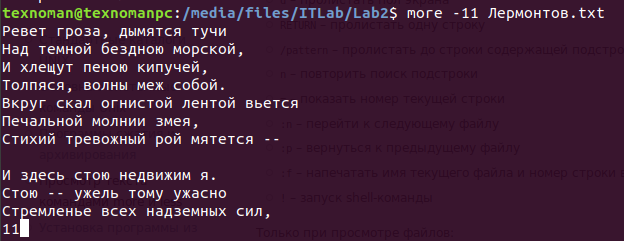
\includegraphics[width=\textwidth]{112.png}
	\\
		\paragraph{4)}
		Выведите этот же текст, используя редактор less. 
		\\
		Для вывода текста стихотворения с использованием \textit{less} вводим 			\textit{less <name>}\\
	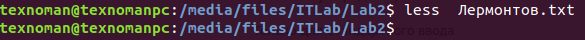
\includegraphics[width=\textwidth]{113(b).png}
	\\
	\begin{center}
		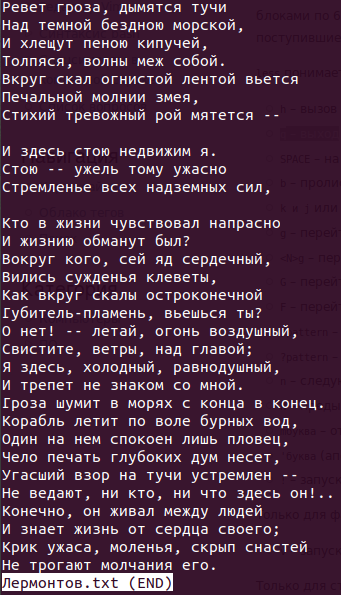
\includegraphics[width=0.65\textwidth]{113(r).png}
	\end{center}
	
		\paragraph{5)}
		Проанализируйте отличия этих редакторов. 
		\\
		В качестве анализа редакторов \textit{more} и \textit{less} можно 				предоствавить различия в просмотре документа: в дополнение к функциям 				\textit{more}  (постраничная или построчная прокрутка текста от начала до конца 	и поиск), команда less позволяет выполнять следующие операции: переход на 			указанную строку(number+g), переход в начало или  конец текста(g/G), прокрутка 		текста от конца к началу, поиск в обратном направлении.\\
		
	\subsection*{6 Управление правами доступа к файлам и каталогам}
	
		\paragraph{1)}
		Вывести полную информацию обо всех файлах из папки «Произведение автора» и файла, извлеченного из архива .zip (п.3 задания 2), и проанализировать выведенную информацию. 
		\\
		Поскольку в 3 пункте 2 задания мы извлекали один файл, о нём и пойдет речь. 	Используем \textit{stat <name>} для вывода полной информации о файле. \\
	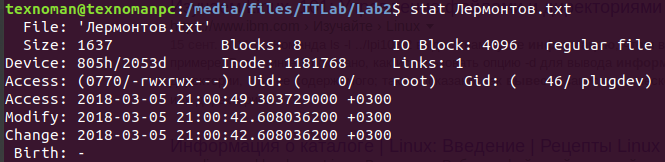
\includegraphics[width=\textwidth]{114.png}
	\\
	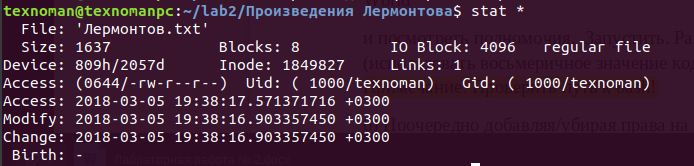
\includegraphics[width=\textwidth]{115.png}
	\\
		\paragraph{2)}
		Удалить права на чтение в одном из произведений. Попытаться вывести на экран. Проанализировать результат. 
		\\
		Удаляем права на чтение в файле Лермонтов.txt, для 			этого вводим \textit{chmod a-r <name> }, где \textit{a-r} означает удаление(-) 		прав у всех (all)  пользователей на чтение (read). Мы не смогли прочесть файл (вывести текст на экран), это связанно с тем, что право на чтение файла было удалено для всех. 
	Прав нет - сделать нельзя.\\
	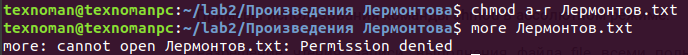
\includegraphics[width=\textwidth]{116.png}
	\\
		\paragraph{3)}
		Удалить права на запись в одном из произведений. Попытаться внести изменения в текст. Проанализировать результат. 
		\\
		Удаляем у файла Лермонтов.txt права на запись. Чтобы это сделать пишем: 		\textit{chmod a-w}, где \textit{a-w} - удалить(-) у всех(all) право на 				запись(write). Проверяем попыткой заменить пробемы на ничего, то есть удалить 		пробелы в тексте произведения. Pедактирование выбранного файла не получилось, потому что ранее были удалены права на изменение. \\
	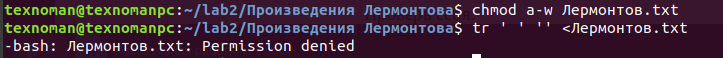
\includegraphics[width=\textwidth]{117.png}
	\\
	
		\paragraph{4)}
		Добавить право выполнения членам группы и остальным пользователям для одного из текстов. Запустить. Проанализировать результат. 
		\\
		Добавляем право выполнения членам группы и остальным  для документа 			Лермонтов.txt . Для этого используем команду \textit{chmod go+x}. Go(group and 		others) +(добавить) x(execute). Мы не можем 'выполнять' файл, поскольку не являемся группой пользователей и/или 'остальными', что можно видеть на изображение. \\
	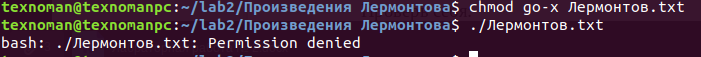
\includegraphics[width=\textwidth]{118.png}
	\\
		\paragraph{5)}
		Создать текстовый файл hello_world.sh с текстом: #!/bin/bash echo "Hello World"
и посмотреть полномочия. Запустить. Разрешить файлу исполнение (использовать восьмеричное значение кода права доступа). Запустить. Примечание: Проверить путь к bash! 
	\\
		Создаём текстовый файл hello\_ world.sh с помощью редактора nano: 				\textit{nano}, прописываем текст \#!/bin/bash echo "Hello World", сохраняем и 		выходим. Выполняем проверку - всё работает, ехууу)) Проверяем путь - вё хорошо.		\\
	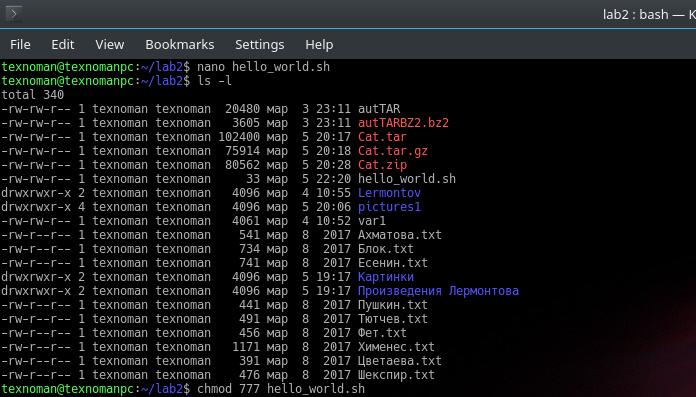
\includegraphics[width=\textwidth]{picture24.png}
	\begin{center}
		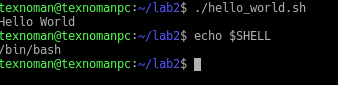
\includegraphics[width=0.7\textwidth]{picture25.png}
	\end{center}
	
		\paragraph{6)}
		Поочередно меняем значения записи/чтения/выполнения, для чего используем 		\textit{chmod} в различные конфигурации. \\
		Файл: \\
		Для чтения нам требуется только право на чтение. Для записи право на запись (право на чтение не обязательно, если знаем название файла и его расположение, также право на использование не обязательно, если собственно использование избегать). Для удаления файла необходимо право на использование (опять же, если мы знаем название файла). Для перемещения и переименования анологично предыдущему описанию.\\
		Директория:\\
		
		\begin{center}
			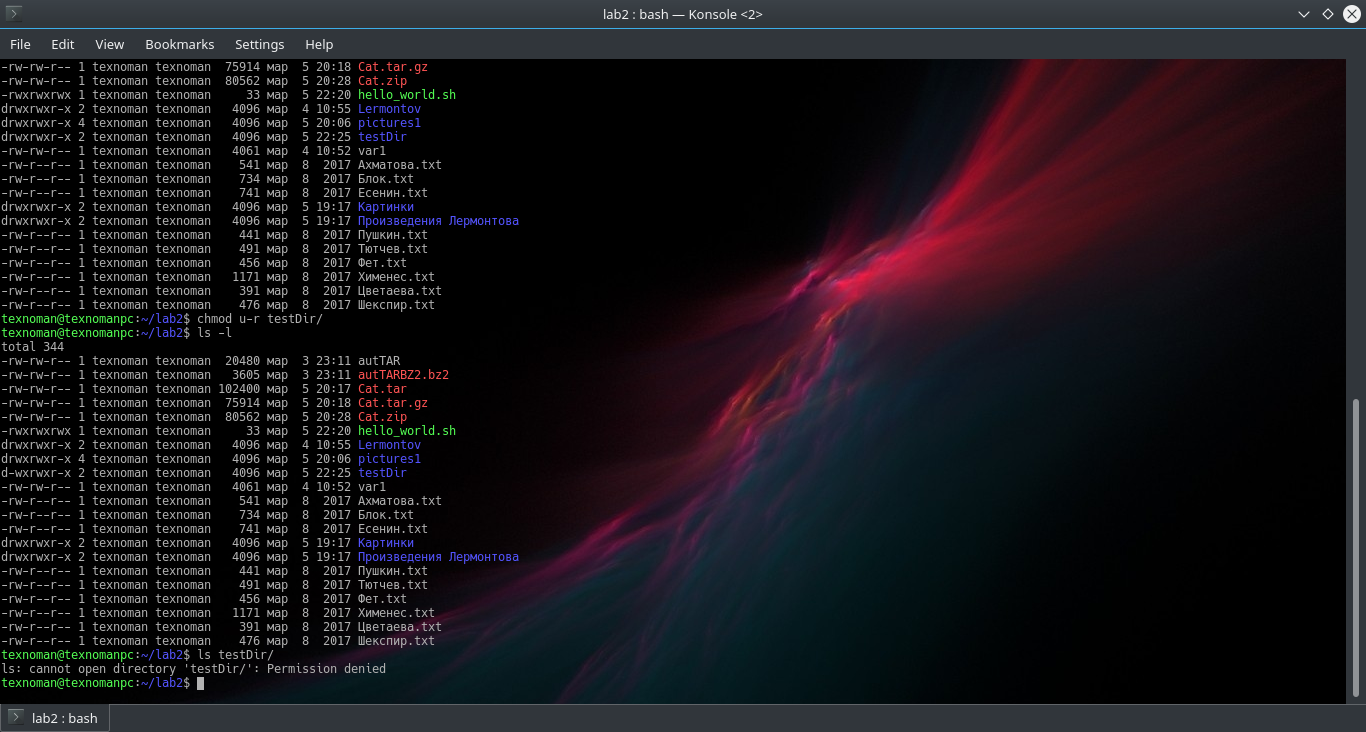
\includegraphics[width=0.7\textwidth]{picture26.png}
		\end{center}
		\vspace{0.1cm}
		\begin{center}
			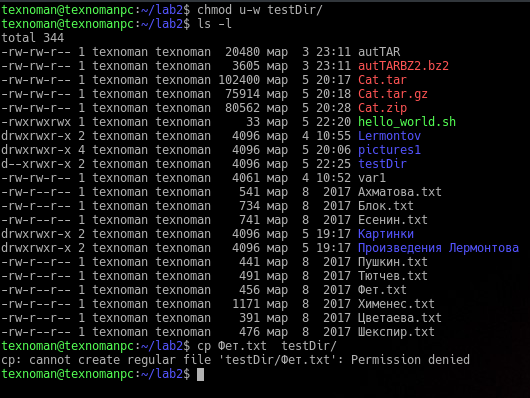
\includegraphics[width=0.6\textwidth]{picture27.png}
		\end{center}


	  
	  
	  
		
